\documentclass[11pt]{beamer}
%\documentclass[handout,dvips,11pt,grey]{beamer}

\usepackage{multicol}
\usepackage{verbatim}
\usepackage{graphicx}
\usepackage{listings}

% ``define'' Scala
\lstdefinelanguage{scala}{
  morekeywords={abstract,case,catch,class,def,%
    do,else,extends,false,final,finally,%
    for,if,implicit,import,match,mixin,%
    new,null,object,override,package,%
    private,protected,requires,return,sealed,%
    super,this,throw,trait,true,try,%
    type,val,var,while,with,yield},
  otherkeywords={=>,<-,<\%,<:,>:,\#,@},
  sensitive=true,
  morecomment=[l]{//},
  morecomment=[n]{/*}{*/},
  morestring=[b]'',
  morestring=[b]',
  morestring=[b]"''
}
\usepackage{hyperref}

\begin{document}

\title{PPAML2015 Summer School}

\subtitle{Geolocation Using Wi-Fi Signal in Figaro}

\author{Sebastian Imlay, Daniel Salvadori, Philip Robinson}

\institute{PPAML}

\date{\today}

\begin{frame}
  \titlepage
\end{frame}


\begin{frame}{Domain Problem}
The end goal of this project is to use wifi power levels to estimate geolocation.

Subproblems
\begin{itemize}
\item Given noisy GPS data, infer ourown location
\item Given our own location and noisy power level readings, infer wireless transmitter location
\item[$\star$] Given our understanding of noisy wifi power data, infer our own relative location {\em (similar to SLAM)}
\end{itemize}
We need to understand
\begin{itemize}
\item attinuation of recieved power levels
\item describe and express models {\em (eg. plate diagrams, PPLs)}
\end{itemize}
\end{frame}

\begin{frame}{Implementation - Figaro}
\begin{multicols}{2}
\resizebox{!}{1.5in}{\lstinputlisting[
    language=scala,
    basicstyle=\footnotesize,
    numbers=left,
    numberstyle=\tiny\color{gray}
  ]{probinso.scala}
}
\columnbreak

\begin{itemize}
\item We all implented our own version of the solution in figaro, and used eachothers solutions to guide us when we got stuck
\item Fist pass we were writing procedural solutions, and our programs didn't really make sence
\item Identifying smaller models, and sculpting data to fit those models helped us think about our problem space
\end{itemize}
\end{multicols}

\end{frame}

\begin{frame}{Model Discussion and History}
\begin{multicols}{3}
\begin{itemize}
\item[N] Transmitters
\item[M] Receivers
\item[S] Receiver Position
\item[X] Receiver Position
\item[A] Attenuation
\item[D] Distance
\item[r] Power
\item[$\hat{r}$]
\end{itemize}
\vfill
\columnbreak

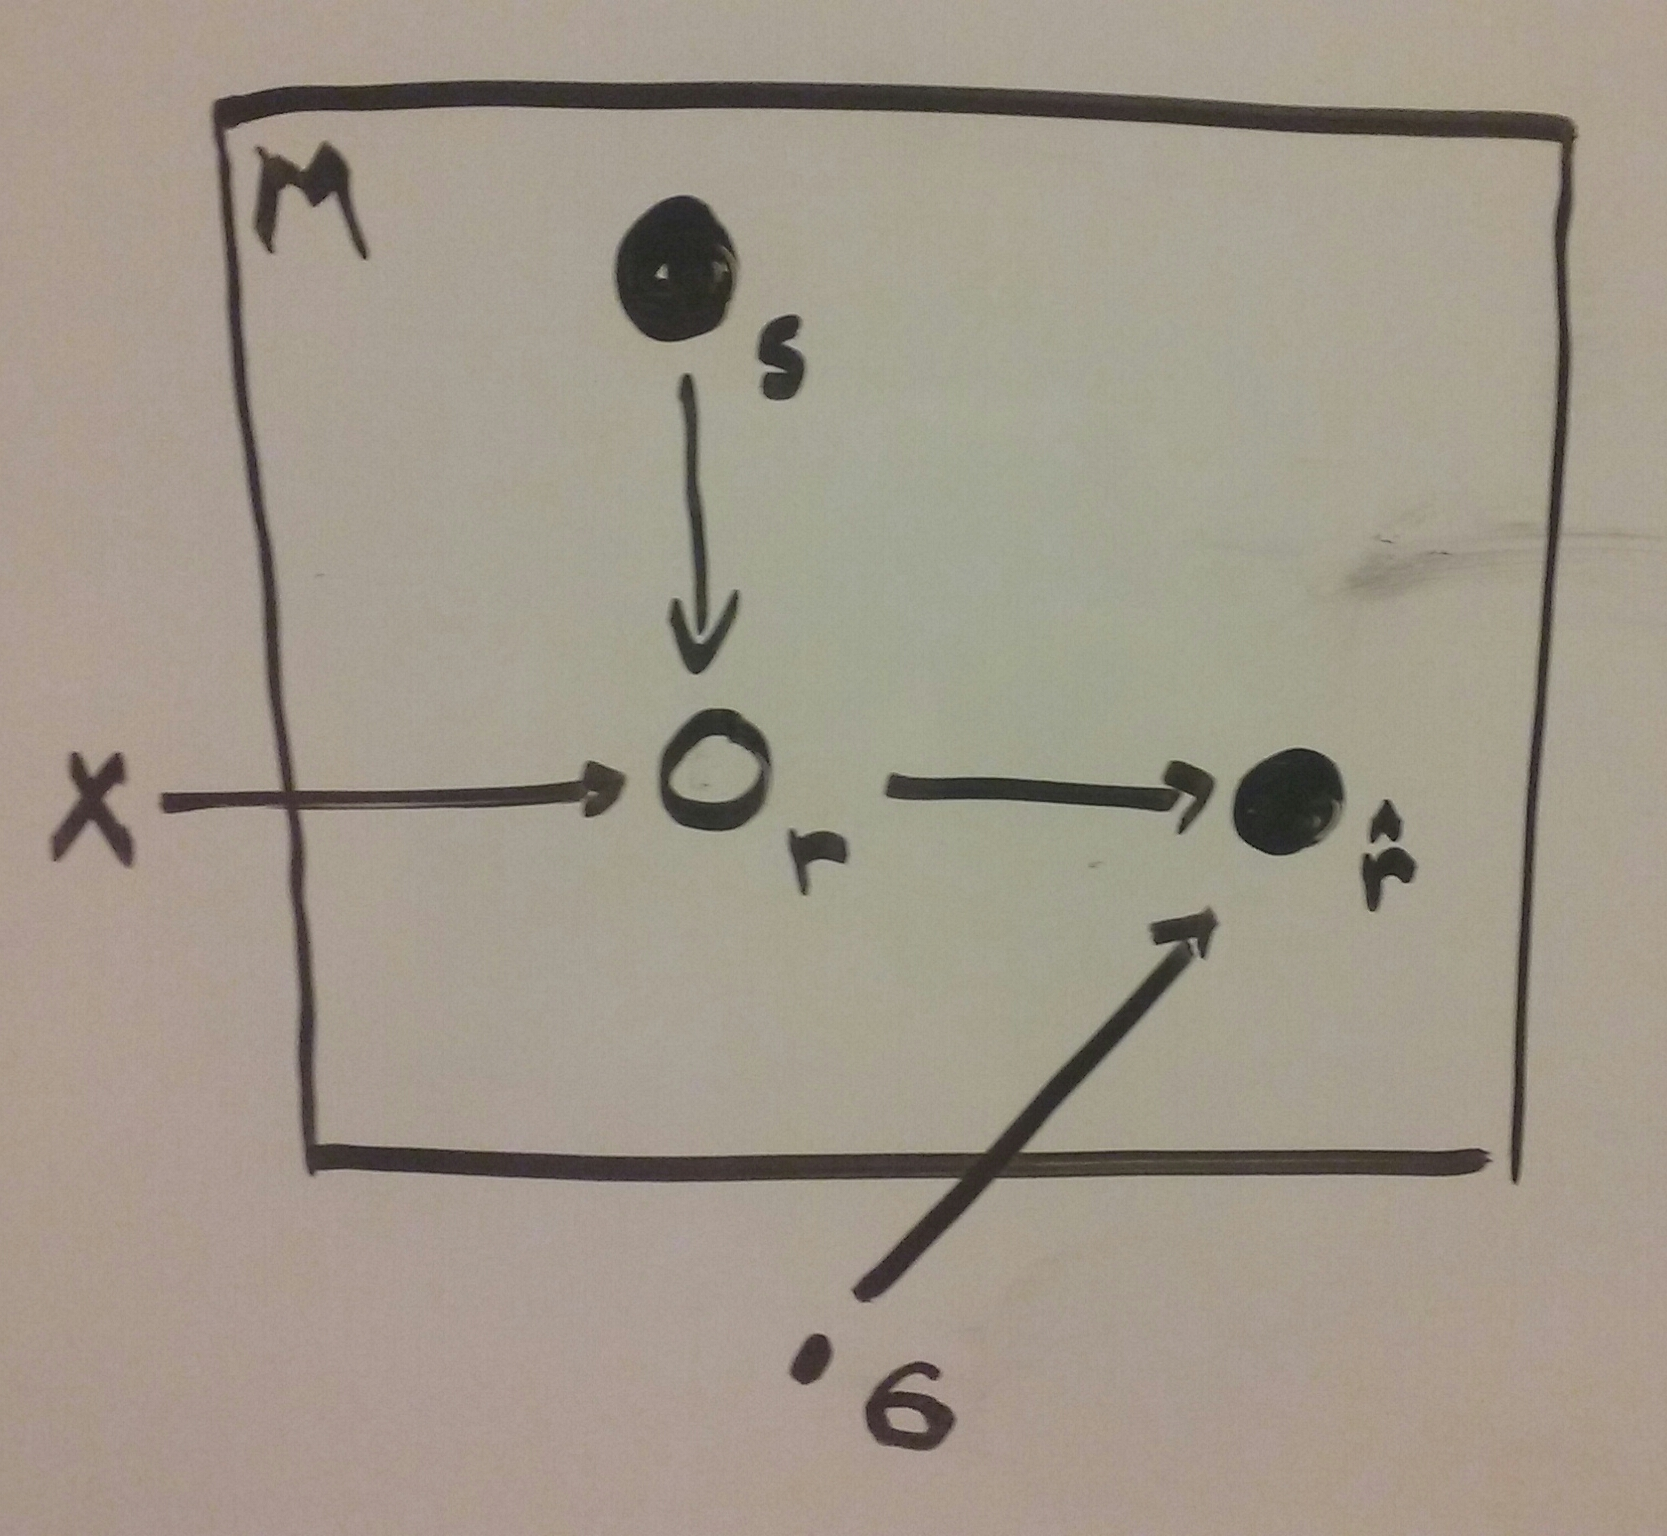
\includegraphics[width=0.3\textheight]{pictures/1plate.jpg}

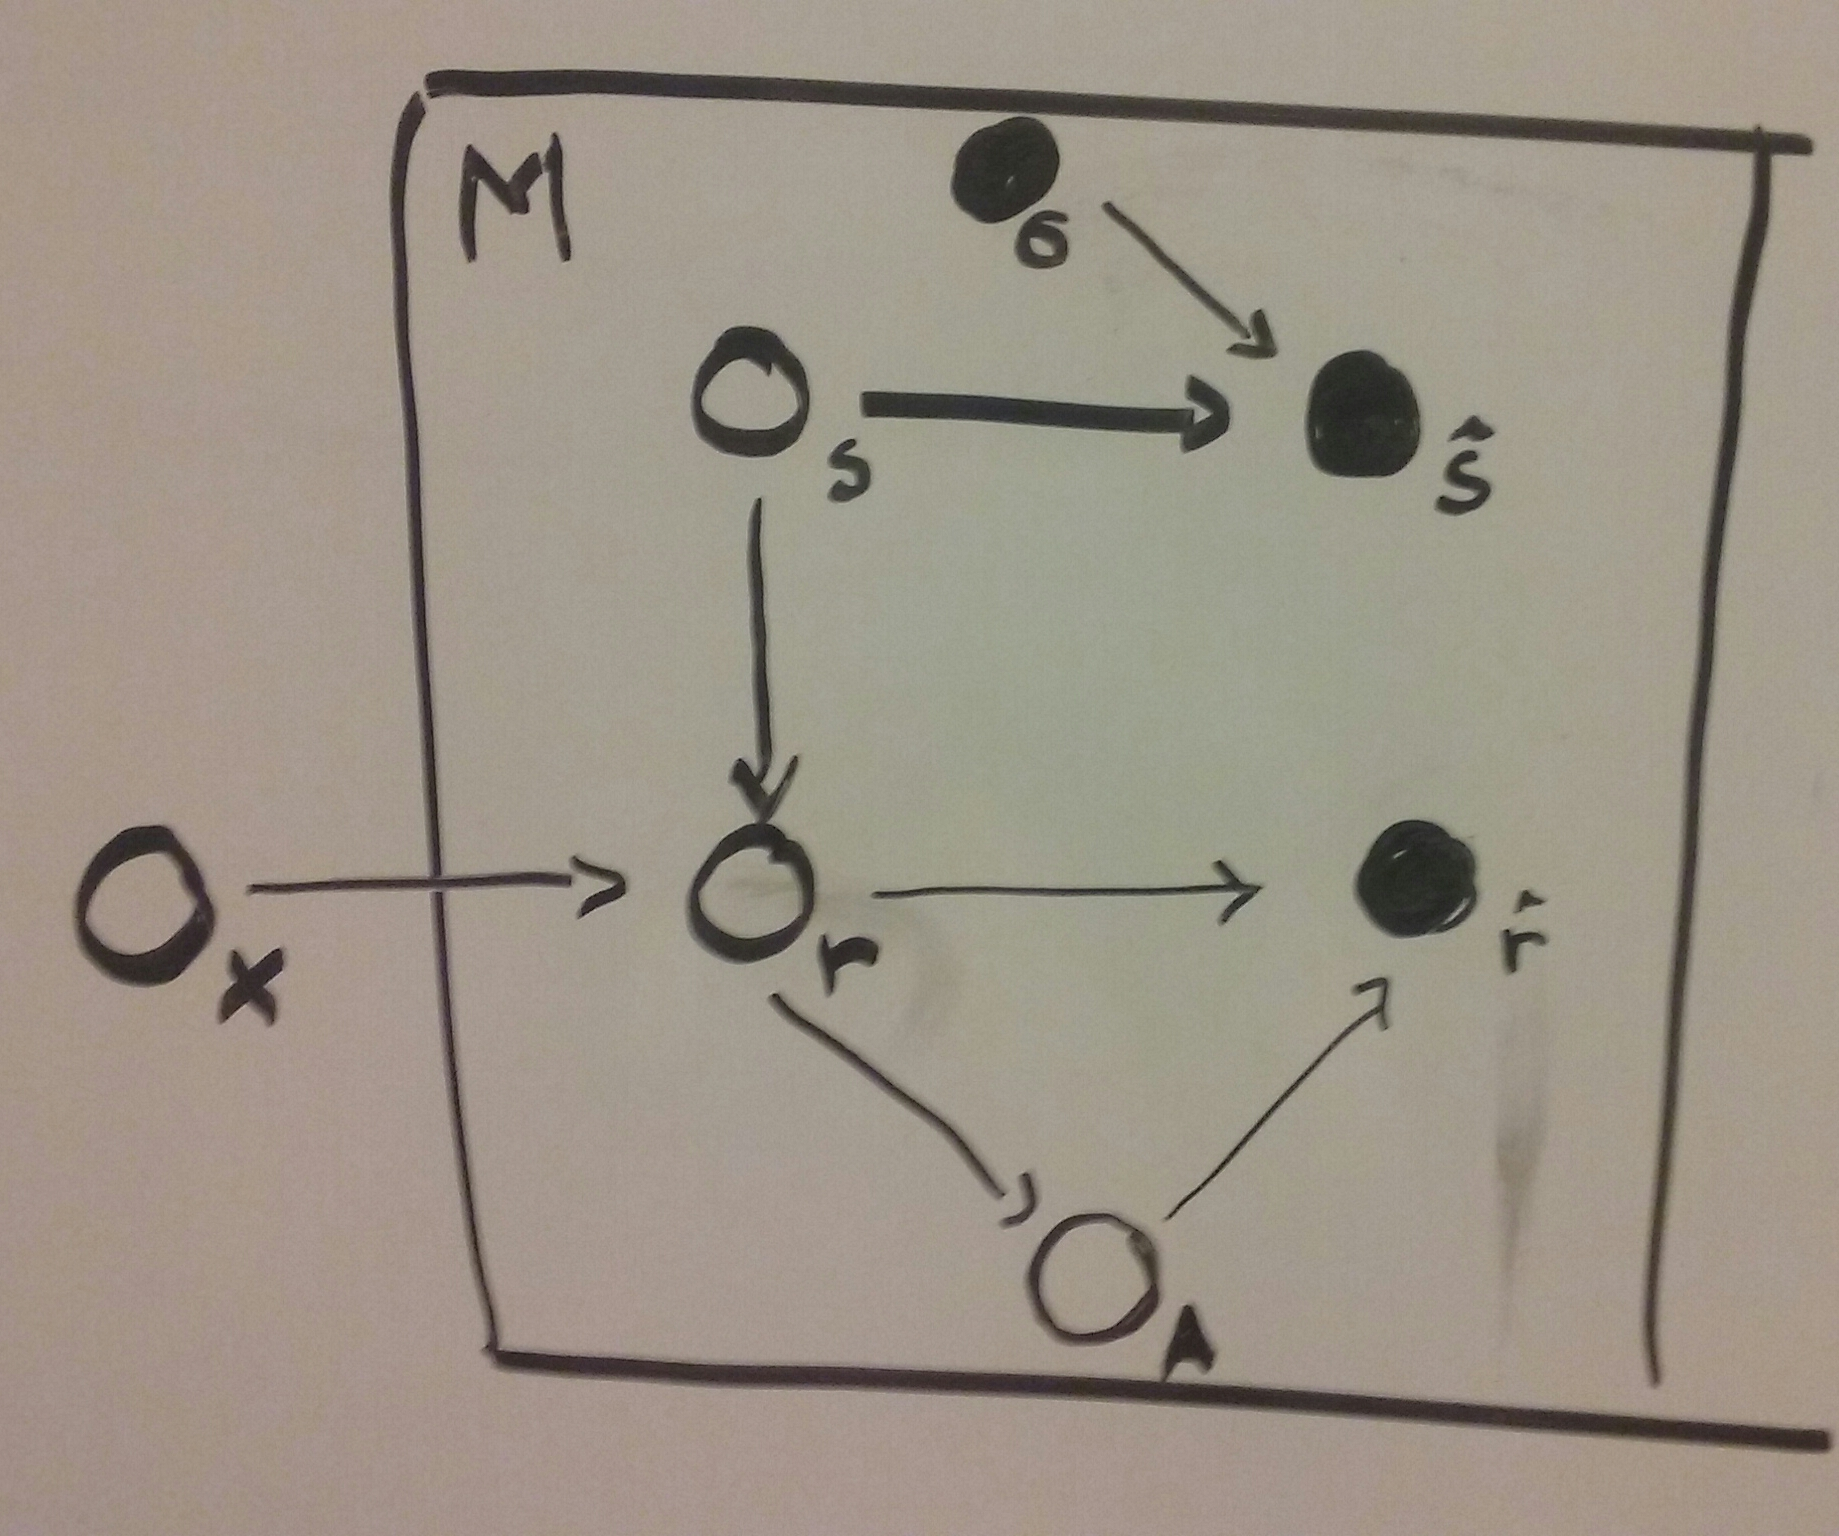
\includegraphics[width=0.3\textheight]{pictures/2plate.jpg}

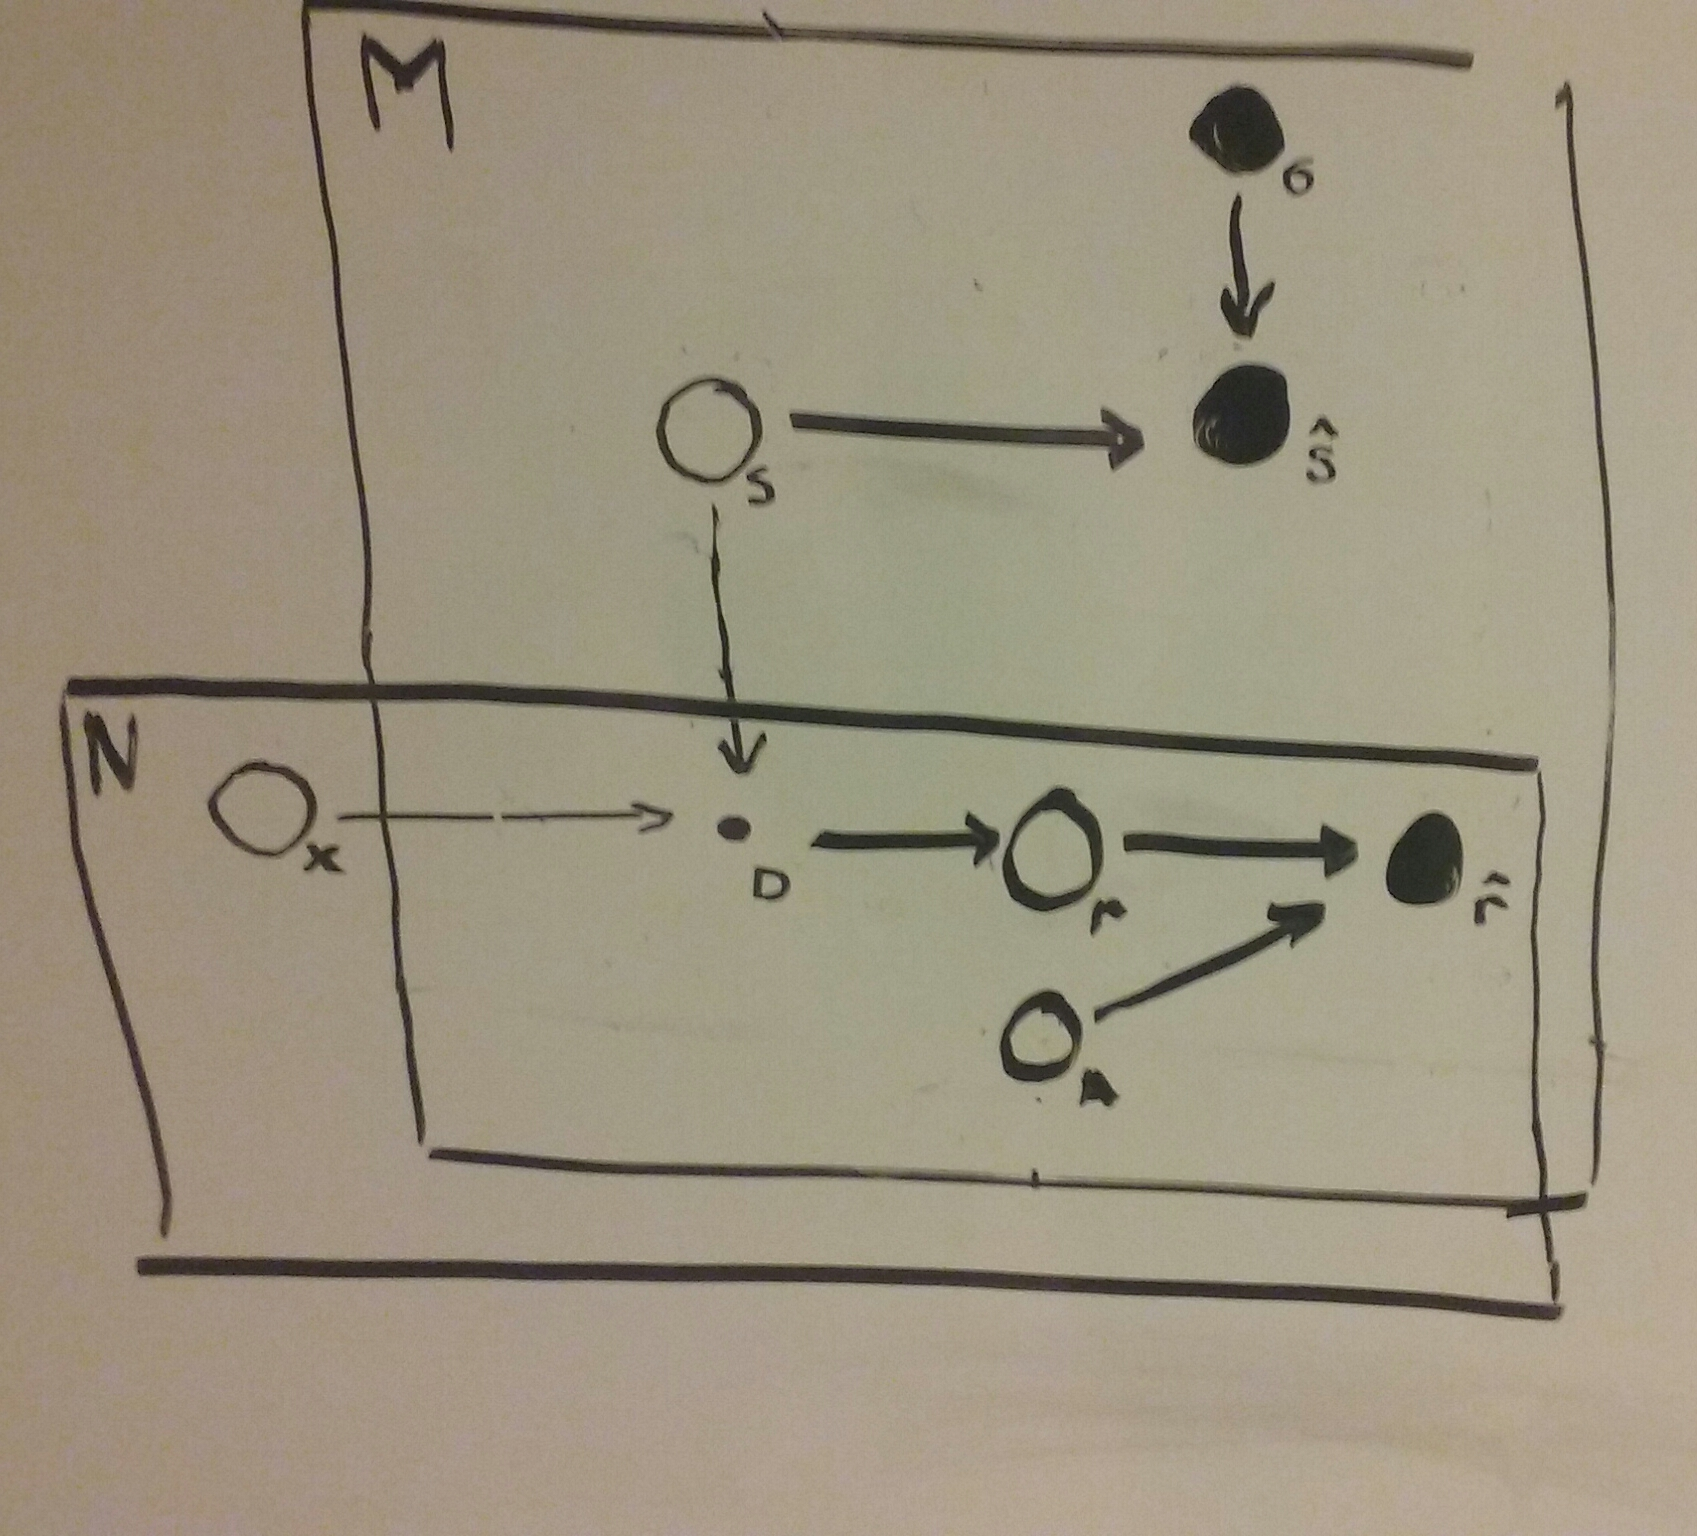
\includegraphics[width=0.3\textheight]{pictures/3plate.jpg}
\vfill\columnbreak

cat
\end{multicols}

\end{frame}



\begin{frame}{Implementation - Supporting Technology}


    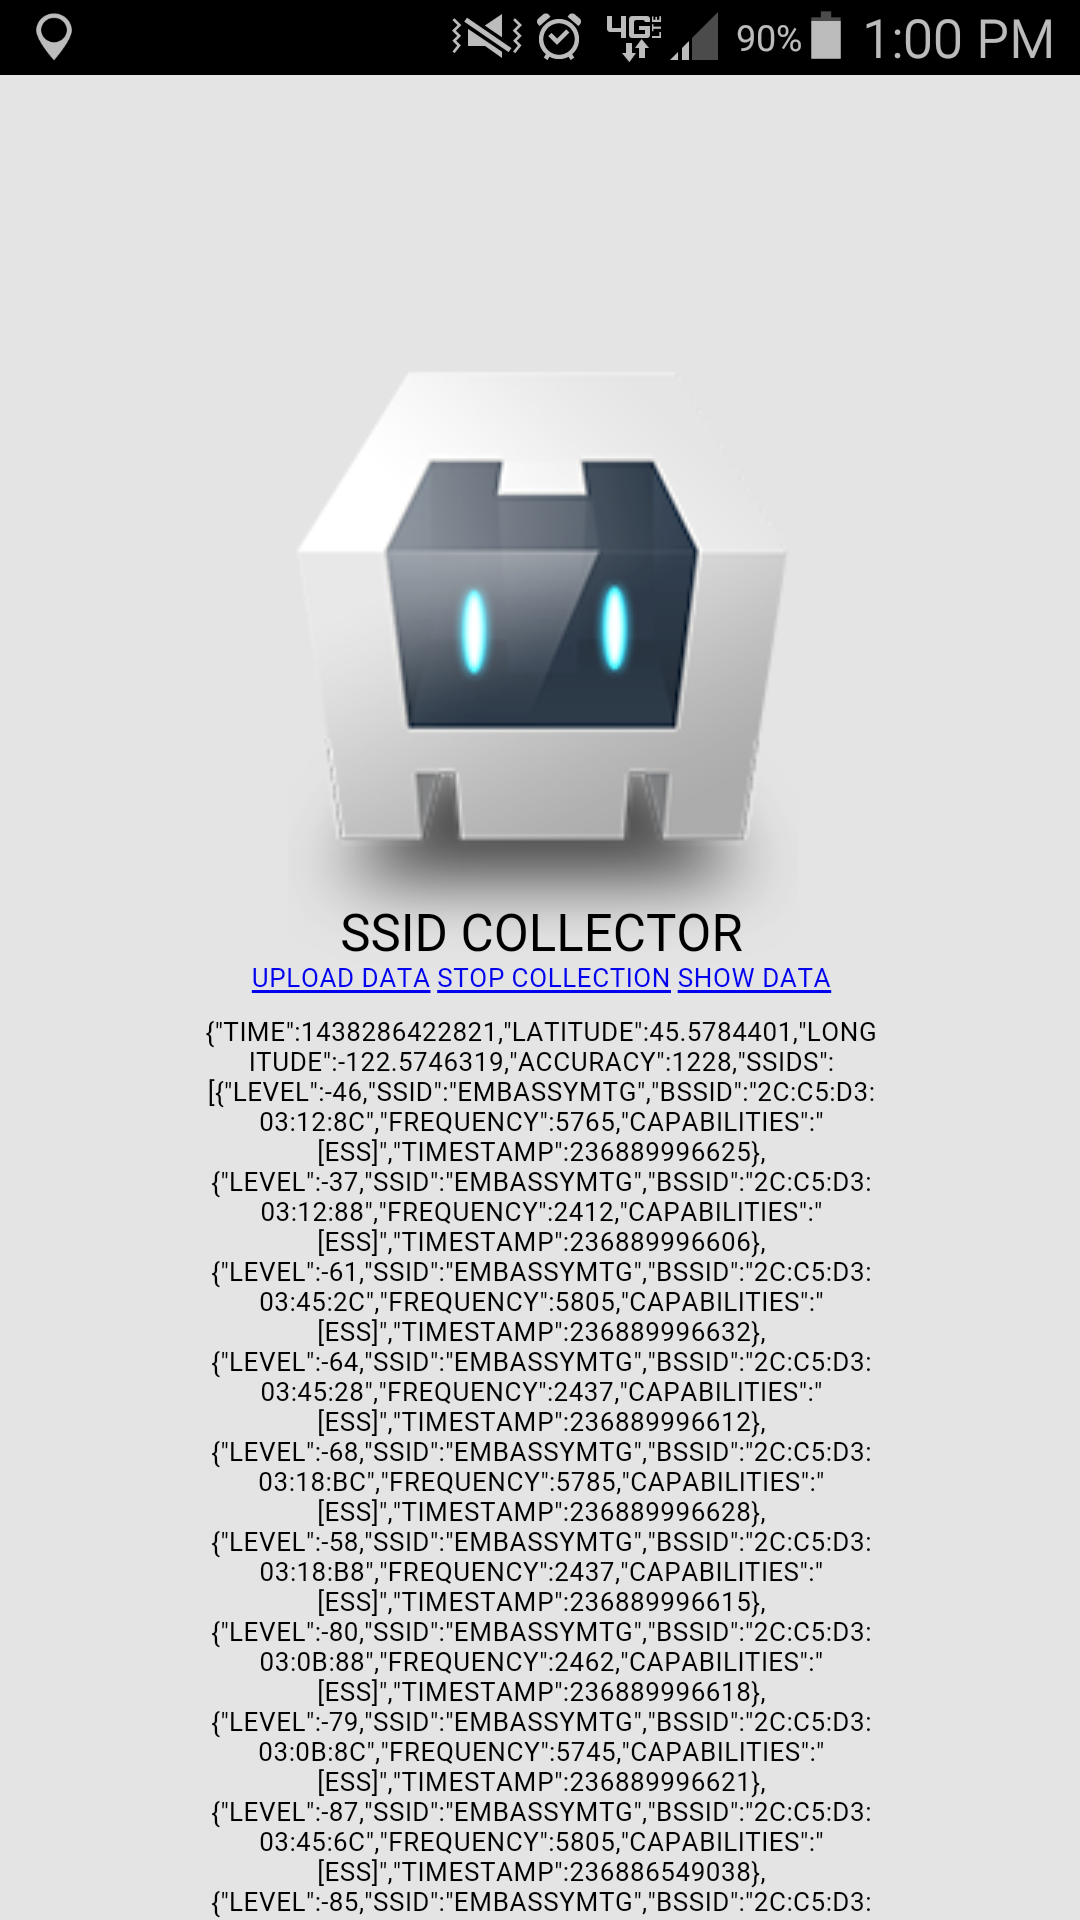
\includegraphics[height=0.7\textheight]{pictures/phoneapp.png}
    \begin{itemize}
        \item Phone app - Apache Cordova
        \item Backend - Couchdb
    \end{itemize}

\end{frame}

\begin{frame}{Interactive Visualization}

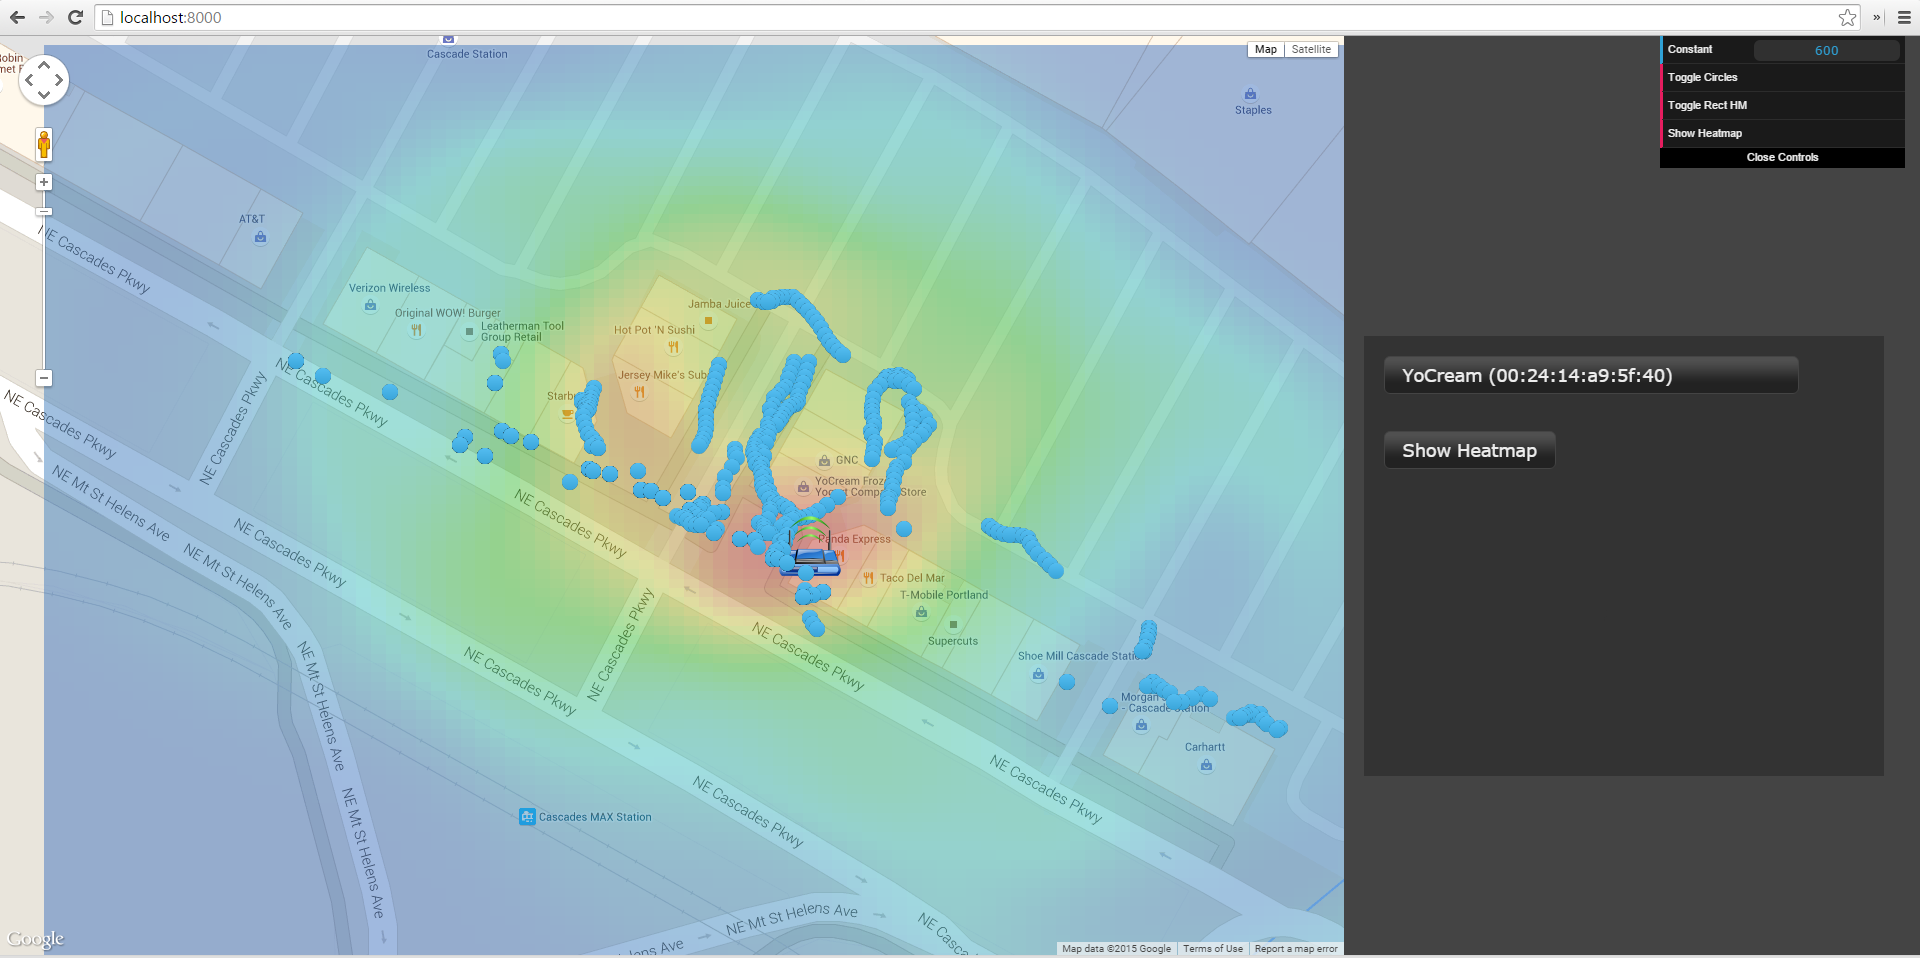
\includegraphics[height=0.55\textheight]{pictures/screenshot4.png}

\href{http://localhost:8000/}{Interactive Visualization Demo}

\end{frame}

\begin{frame}{Collateral}
\href{https://github.com/simlay/wifi-collection}{git repository}
\begin{itemize}
\item data gathering
\item data shaping
\item visualization
\item figaro solutions
\item presentation
\end{itemize}

\end{frame}

\end{document}
